\section{Използвани езици и технологии}

\subsection{Rust}
Rust е програмен език от високо ниво създаден през 2006 година от Graydon
Hoare, който по това време работи за Mozilla. През 2009 година разработката на
езика бива спонсорирана от Mozilla, a през 2010 езика е обявен публично.
\cite{Rust_Origins_Wikipedia}

\subsubsection{Отличаващи се особености на езика}
% Rust е порграмен език от високо ниво, но това не му пречи да е почти толкова
% бърз колкото езици от по-ниско ниво като C/C++.

Езици като C\#, Python и JavaScript използват система за освобождаване на паметта
наречена Garbage Collector (GC). За да може да се освободят неизползваните
променливи, изпълнението на програмата трябва да бъде спряно на пауза и да се
провери дали има заделени региони от паметта, към които вече не се използват
или са маркиране за освобождаване от програмиста \cite{Garbage_Collection_Wikipedia}.

Rust използва система наречена borrow checker, която проверява, по време на
компилация, дали програмата следва следните принципи:

\begin{itemize}

\item Ресурсите (отделената памет за стойноста) могат да имат само един
собственик и това е самата промелива. Когато променлива вече не може да бъде
достъпена ресурсите биват освободени.

\item Когато една променлива бъде подадена към някоя функция, собственик на
ресурсите става функцията. Ако се пробваме подадем отново променливата,
компилатора ще ни каже, че променливата е била преместена (Use of moved value).
\begin{figure}[!htb]
  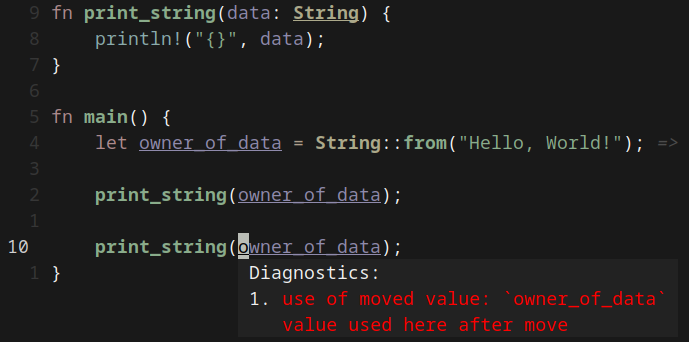
\includegraphics[width=\textwidth,keepaspectratio=true]{rust-use-after-move}
  \centering
  \caption{Модела на собственик в Rust}
  \label{fig:rust-use-after-move}
\end{figure}

\end{itemize}

\subsubsection{Enum}
Enum е един от основните типове в Rust. Всеки вариянт на enum-а може да има
съдържа информация от различен вид \cite{Rust_Enums}. Така са имплементирани
някои от най-важните типове: Option<T> и Result<T, E>.

\begin{figure}[!htb]
  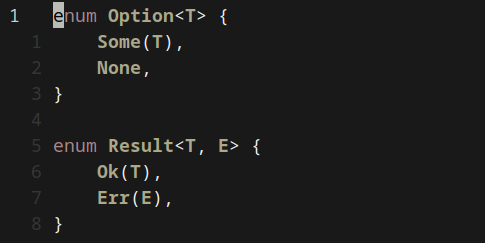
\includegraphics[scale=0.75]{rust-enum-example}
  \centering
  \caption{Стандартната имплементация на Option<T> и Result<T, E>}
  \label{fig:rust-enum-example}
\end{figure}

\newpage

\subsubsection{Option типа}
В повечето езици съществува идеята за NULL пойнтери. Когато един pointer е Null
това означа, че той сочи към нищо. Идеята за Null на теория е много добра, но
на практика създава повече проблеми. Ако се пробваме да достъпим pointer който
е Null, програмата ще крашне или в някои езици като C\# ще хвърли
NullReferenceException.

Разработчиците на Rust са намерили много добър заместител на Null и това е
Option enum-а, който има два варинта. Това са Some(T) когато имаме някаква
стойнос и None когато нямаме нищо.

\subsubsection{Result типа}
Когато програмираме на C\# много често ни се случва да хвърляме Exception-и и
съответно да ги хващаме с try/catch блока. Еxception-ите се ползват когато в
една функция възникне грешка.

Във Фигура \ref{fig:csharp-exceptions-1-code} е даден код който на пръв поглед
изглежда добре, но има скрити бъгове. Какво ще стане ако потребилтеля въведе
дума вместо число? Ще получим Exception който ни казва: "Input string was not
in a correct format".
\begin{figure}[!htb]
  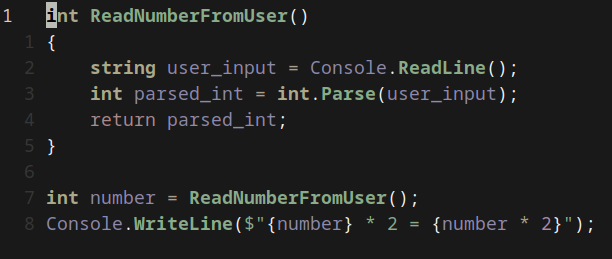
\includegraphics[scale=0.75]{csharp-exceptions-1-code}
  \centering
  \caption{Пример за скрит Exception}
  \label{fig:csharp-exceptions-1-code}
\end{figure}

\begin{figure}[!htb]
  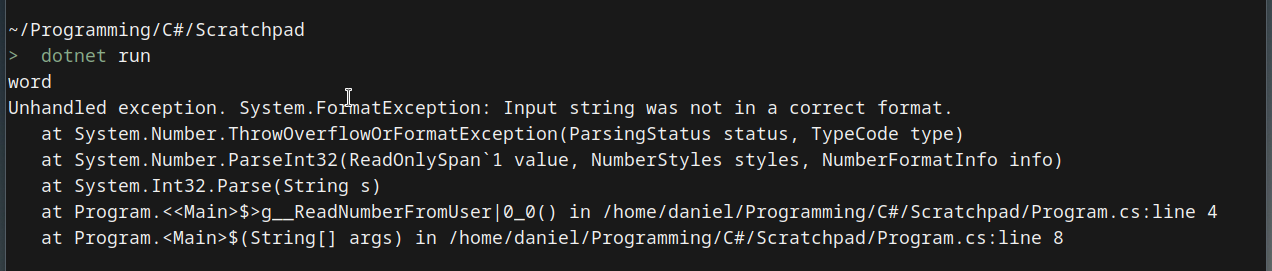
\includegraphics[width=\textwidth,keepaspectratio=true]{csharp-exceptions-1-output}
  \centering
  \caption{Изход на кода от Фигура \ref{fig:csharp-exceptions-1-code}}
  \label{fig:csharp-exceptions-1-output}
\end{figure}

Проблема е че ние като програмисти не знаем, че int.Parse може да хвърли
Exception без да се консултираме с документацията \cite{CSharp_Int_Parse}.
Същият код написан на Rust би изглеждал по следния начин [Фигура \ref{fig:rust-exceptions-1-code}].

\begin{figure}[!htb]
  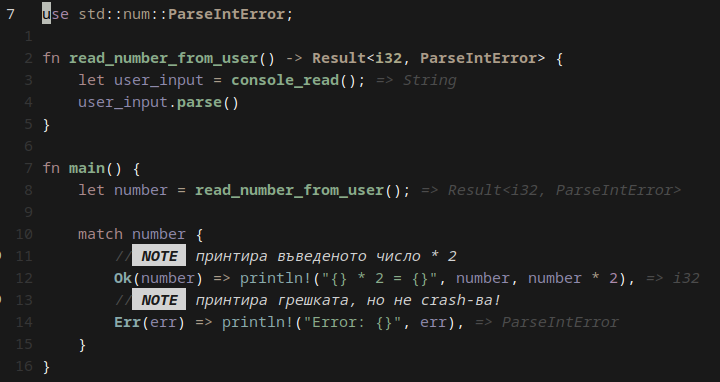
\includegraphics[scale=0.60]{rust-exceptions-1-code}
  \centering
  \caption{Кода от Фигура \ref{fig:csharp-exceptions-1-code} написан на Rust}
  \label{fig:rust-exceptions-1-code}
\end{figure}

Разликата между C\# и Rust е че Rust кода ни кара ни показва типовете при успех
и грешка. Функцията връща променлива от тип Result<T, E> където T е
променливата от тип i32 (int) ако всичко се и изпълнило без проблем, а E е от
тип ParseIntError.

За да използваме резултата от функцията, какъвто и да е той, можем да
използваме match. С match можем да проверим дали резултата е Ok или Err.


% \subsection{PDF}
% PDF е файлов формат създаден от Adobe през 1992г. предназначен да бъде преносим
% документ, независим от хардуера и софтуера. Всеки един PDF файл съдържа пълно
% описание на начина по който трябва да изглежда документа \cite{PDF_Wikipedia}.
%
% \subsubsection{Технически детайли}
% PDF най-често е комбинация от векторни графики и текст.
%
% В по-нови ревизии на PDF станзарта, документите могат да имат линкове които можем да отворим и подръжка за plugin-и.

\newpage
\subsection{egui}
egui е проста, бърза и много преносима библиотека за графични потребителски
интерфейси (GUI). Тя работи на много платформи включително: уеб браузъри, като
обикновено приложение или в някои game engine-а. Написана е на Rust и има много
лесен и интуитивен API за разработване.

Главните цели на проекта са:
\begin{itemize}
    \item Най-лесната за използване GUI библиотека;
    \item Отзивчив: цели поне 60 FPS при компилация с Debug опциите;
    \item Преносим: кодът да работи в браузър и като собствено приложение;
    \item Лесен за интегриране във всяка среда;
    \item Модулен: можете да използвате малки части от egui и да ги комбинирате
    по нови начини \item Минимален брой завивисимости (библиотеки)..
\end{itemize}

\subsubsection{Минимален пример}
egui библиотеката ни дава достъп до \textit{eframe::App} интерфейса. Този интерфес съдържа една
функция \textit{update}. Тя се извиква всеки пътр когато потребителският интерфейс се е
променил или се получи някакво събите (Event) от мишката или клавиатурата. 
[Фигура \ref{fig:egui-example-1}]

\begin{figure}[!htb]
  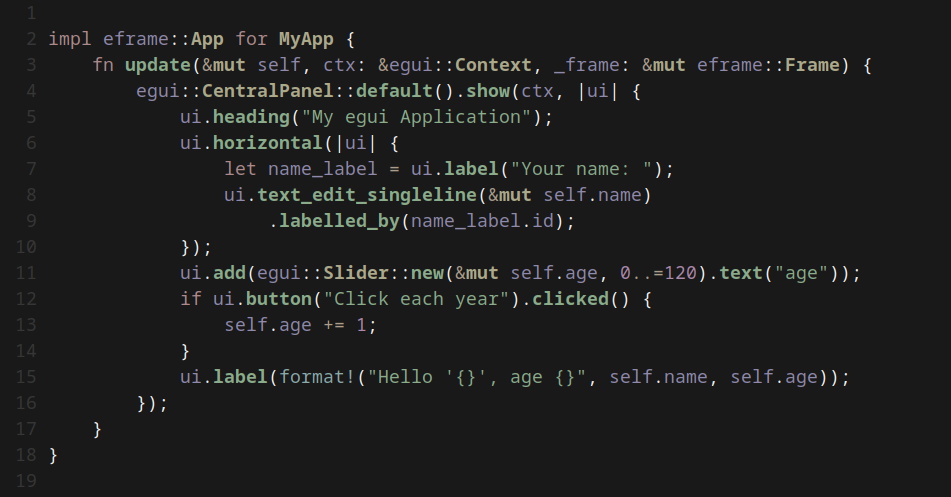
\includegraphics[width=\textwidth,keepaspectratio=true]{egui-example-1}
  \centering
  \caption{Имплементация на egui интерфейса}
  \label{fig:egui-example-1}
\end{figure}

Библиотеката е достатъчно умна сама да прецени дали се нуждае от повторно
изобразяване, или не.

egui е GUI библиотека от незабавен режим (Immediate Mode). Това означава, че
начина, по който искаме да изглежда графичния интерфейс, се описва, извиквайки
методи. По този начин се упростява разработката на графичния интерфейс. За да покажем един прост
бутон се нуждаем от един if оператор.


\subsection{genpdf}
genpdf е библиотека която абстрахира създаването на PDF файлове. Тя се грижи за
оформлението на страницата, подравняването на текста и изобразяването на
структурата на документа в PDF файл. Библиотека както и всичките и зависимости
са написани на Rust и следват добрите практики на езика
\cite{genpdf_repository}.

\subsubsection{Елементи}
genpdf използва елементи за да опише оформлението на документа. Всеки елемент
имплементира Element интерфейса. Интерфейса съдаржа функция render която бива
извикана всеки път когато елемента трябва да бъде показан в PDF файла
\cite{genpdf_element_trait}.

Използвайки Element интерфейса, разработчиците на genpdf са ни предоставили
най-често използваните елементи:
\begin{itemize}
    \item Контейнери:
        \subitem LinearLayout: подрежда елементите си последователно
        \subitem TableLayout: подрежда елементите си в колони и редове
        \subitem OrderedList/UnorderedList: подредете елементите им последователно с bullet-и
    \item Текст:
        \subitem Text: един ред текст
        \subitem Paragraph: подравнен параграф
    \item Обвивки:
        \subitem FramedElement: елемент с рамка
        \subitem PaddedElement: добавя разтояние между елементите
        \subitem StyledElement: задава стил по подразбиране за обвития елемент и неговите деца
    \item Други:
        \subitem Image: снимка с описание
        \subitem Break: добавя прекъсвания на редове като разделител
        \subitem PageBreak: добавя принудително прекъсване на страницата
\end{itemize}


\newpage

\section{Подготовка}
Преди да започнем с разработката на софтуера трябва да настроим нашата среда за
действието. Тя включва Rust компилатора, текстов редактор (IDE) и Git за
контрол на версиитe.

% LLVM is a set of compiler and toolchain technologies that can be used to
% develop a front end for any programming language and a back end for any
% instruction set architecture. LLVM is designed around a language-independent
% intermediate representation (IR) that serves as a portable, high-level assembly
% language that can be optimized with a variety of transformations over multiple
% passes. The name LLVM originally stood for Low Level Virtual Machine, though
% the project has expanded and the name is no longer officially an acronym. 
\subsection{Инсталиране на Rust}
Rust е език който използва LLVM за обръщането на код в машинни инструкции.
LLVM е набор от технологии за компилиране, който позволява да бъдат написани
различни frontend-ове за всеки език и backend-ове за всяка хардуерна архитектура.
Благодарение на този факт Rust може да работи на всички модерни операционни системи
като Windows, MacOS, Linux, OpenBSD и още много други.

За операционните систтеми базирани на UNIX принципите, като MacOS и Linux можем
да инсталираме Rust с една проста команда:
\begin{lstlisting}
curl --proto '=https' --tlsv1.2 -sSf https://sh.rustup.rs | sh
\end{lstlisting}

Или през package manager-а на операционната система.
В MacOS това е homebrew.
% TODO: give homebrew install guide

A в Linux зависи от дистрибуцията:
\begin{itemize}
\item Arch Linux - pacman -S rustup
\item Debian Linux - apt-get install rustup
\item Fedora Linux - dnf install rust cargo
\end{itemize}

% TODO: mention WSL
За да инсталираме Rust на Windows трябва да изтеглим 64 или 32 битовия
инсталационен файл от сайта на Rust: https://rustup.rs/. 

\begin{figure}[!htb]
  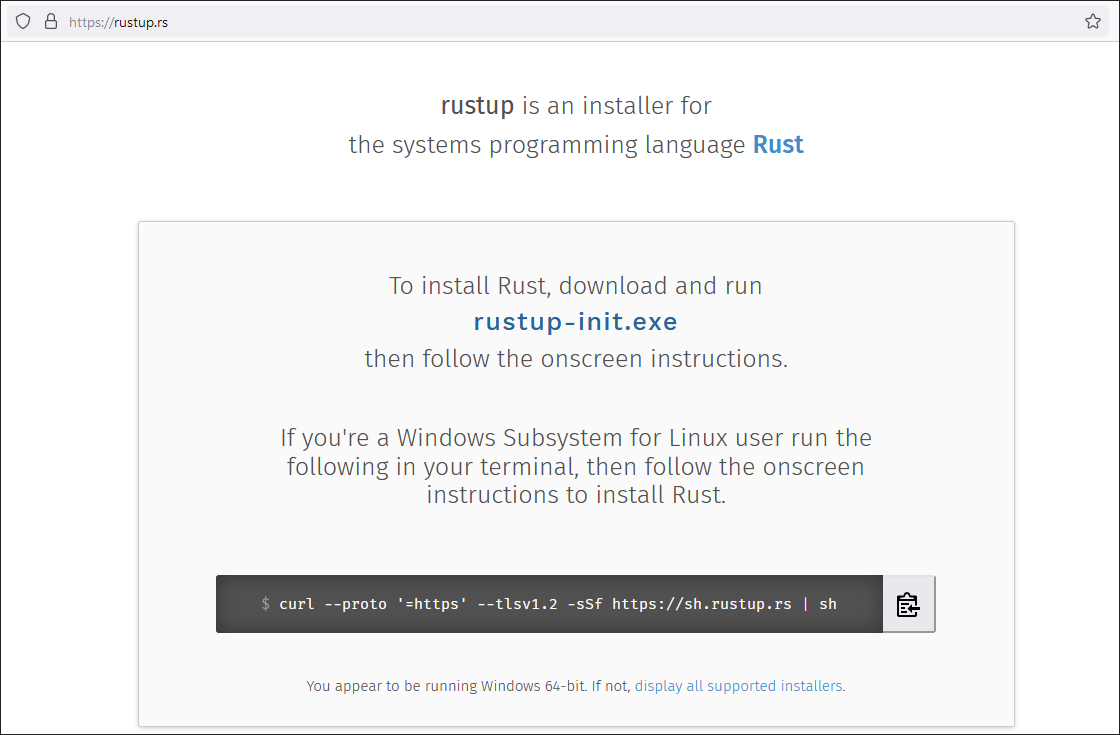
\includegraphics[scale=0.32]{rust-up-windows-install}
  \centering
  \caption{Сайт за изтегляне на инсталационния файл на Rust}
  \label{fig:rust-up-windows-install}
\end{figure}

\newpage
\subsection{Избор на IDE}
За да можем да създаваме софтуер на Rust, по най-ефективния начин се нуждаем от
текстов редактор който поддържа LSP. LSP или Language Server Protocol е
протокол създаден от Microsoft за Visual Studio Code и служи за комуникация
между техтовят редактор и специализирани програми, които анализират кода който
пишем и показват къде има грешки, предложения как да бъдат поправени, допълване
на код, подчертаване на синтаксиса \cite{lsp_wikipedia}.

\subsubsection{Visual Studio Code}
Visual Studio Code е текстов редактор с отворен код създаден от Microsoft. Той
използва Electron за графична библиотека и работи на Windows, Linux и MacOS. 
През 2022 в допитване до потребителите на Stack Overflow, Visual Studio Code е
класиран като най-популярният текстов редакор сред 71 010 респонденти
\cite{vscode_wikipedia}.

% TODO: info about plugins: rust-analyzer etc.

Един от недостатъцине на VSCode обаче е високите системни изисквания за
нормална работа и моментално време за реакция при въвеждане на текст.
\begin{figure}[!htb]
  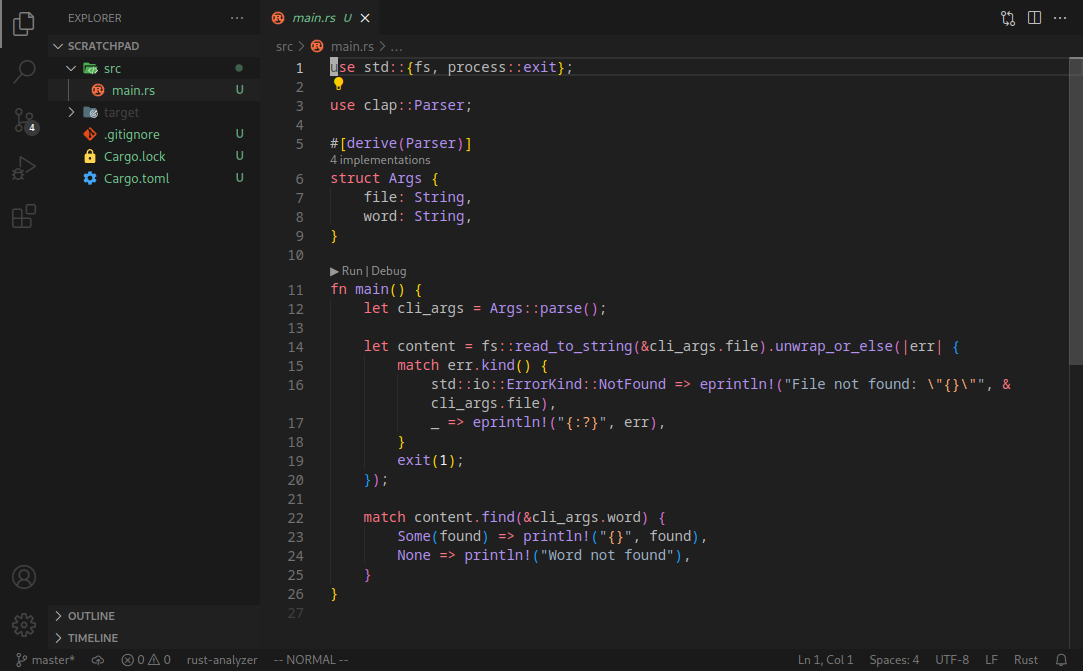
\includegraphics[scale=0.40]{vscode}
  \centering
  \caption{Visual Studio Code}
  \label{fig:vscode}
\end{figure}

\subsubsection{Vim}
Vim e техтов редактор с отворен код първоначално написан за настолният компютър
Amiga\cite{amiga_wikipedia} през 1991 година от Брам Моленар. За разлика от
Visual Studio Code, vim e текстов редактор, който e бил замислен да работи не
само в графичти среди, но и в терминални среди \cite{vim_wikipedia}. 

Най-привекателната част от Vim е начина за навигация. В повечето редктори се
навигира чрез мишката и няколко клавишни комбинации, докато Vim използва само
клавишни комбинации. По този начин ръцете ни остава на клавиатурата и няма
нужда да отделяме време за навигиране с мишка. 

Vim разполага с 3 режима за работа и това са:
\begin{itemize}
\item Normal - В нормалният режим можем само да манипулираме текст
\item Visual - В визуалният режим можем да избираме по-голими региони от текст
\item Command - В командният режим можем да изпълняваме команди за манипулиране
на текст, настройване на редактора и изпълнение на команди в операционната
система \end{itemize}

Vim успява да много малко ресурси от VSCode, без да прави компромиси от към
функционалности. За да може да бъде постигнато Vim е написан на C и потребителя
трябва ръчно да си настрои редактора, използвайки специално направеният език
VimScript. Този процес е прекалено сложен за повечето потребители затова те
предпочитат да използват VSCode, дори и да използва повече ресурси.

\subsubsection{Neovim}
Neovim е копие на Vim, което се стреми да подобри скороста и поддръжката на
Vim. Някои добавени функционалности на копието включват вградена поддръжка на
LSP и поддръжка за Lua скриптове като заместител на VimScript \cite{neovim_wikipedia}.

Проектът Neovim стартира през 2014 година, като някои членове на Vim общността
предлагат помощ в усилията за основно рефакториране, за да осигурят по-добри
eзици за скриптове, плъгини и интеграция с модерни графични потребителски интерфейси.
Проектът е с отворен код и, който е достъпен в GitHub. \cite{neovim_github}

От към производителност Neovim е малко по-бавен от предшественика си Vim, но
все пак е в пъти по-бърз от главния си конкурен Visual Studio Code, затова аз
се спрях на Neovim.

\begin{figure}[!htb]
  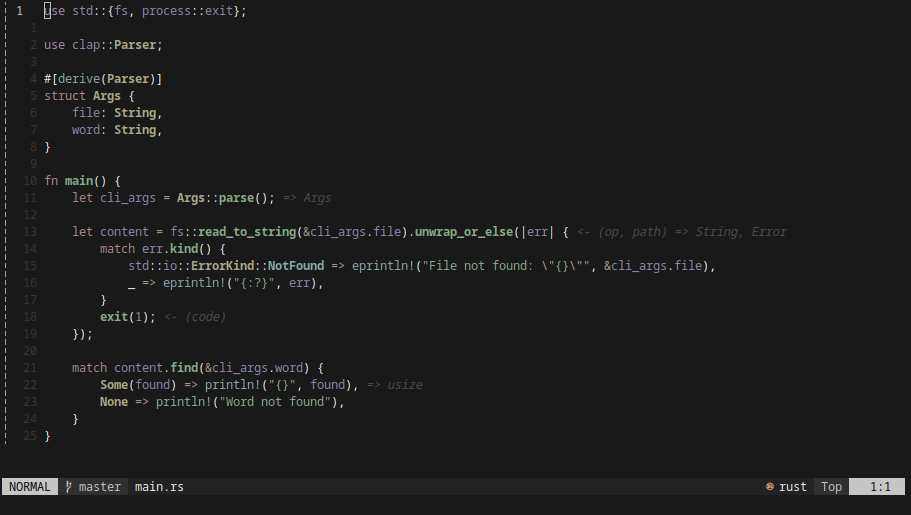
\includegraphics[scale=0.50]{neovim}
  \centering
  \caption{Neovim}
  \label{fig:neovim}
\end{figure}

\subsection{Git}
% TODO: :')

\subsection{Git}
Git е система за контрол на версиите, която проследява промените във всеки
набор от компютърни файлове, обикновено се използва за координиране на работата
между програмистите, които съвместно разработват изходния код по време на
разработката на софтуер. Целите на системата включват скорост, цялост на
данните и поддръжка за разпределени, нелинейни работни потоци (хиляди паралелни
клонове, работещи на различни системи).

Git първоначално е създаден от Линус Торвалдс, през 2005 година за разработване
на ядрото на Linux, като инструмен за други разработчици на ядрото да
допринасят за първоначалното му развитие. От 2005 година Junio Hamano е основният
разработчик. Както при повечето други разпределени системи за контрол на версиите
и за разлика от повечето системи клиент-сървър, всяка Git директория на всеки
компютър е пълноценно хранилище с пълна история и пълни възможности за
проследяване на версиите, независимо от достъпа до мрежата или централен
сървър. Git е безплатен софтуер с отворен код, разпространяван само под лиценз
GPL-2.0. \cite{git_wikipedia}

Git е конзолно приложение, но съсществуват и приложение с графичен интерфейс
като GitHub Desktop. Това приложение ни дава възможност да управляваме
разработката на проекта, създаване на потребителски истории и тяхното
менежиране. [Фигура \ref{fig:github-desktop}] \cite{github_desktop}

\begin{figure}[!htb]
  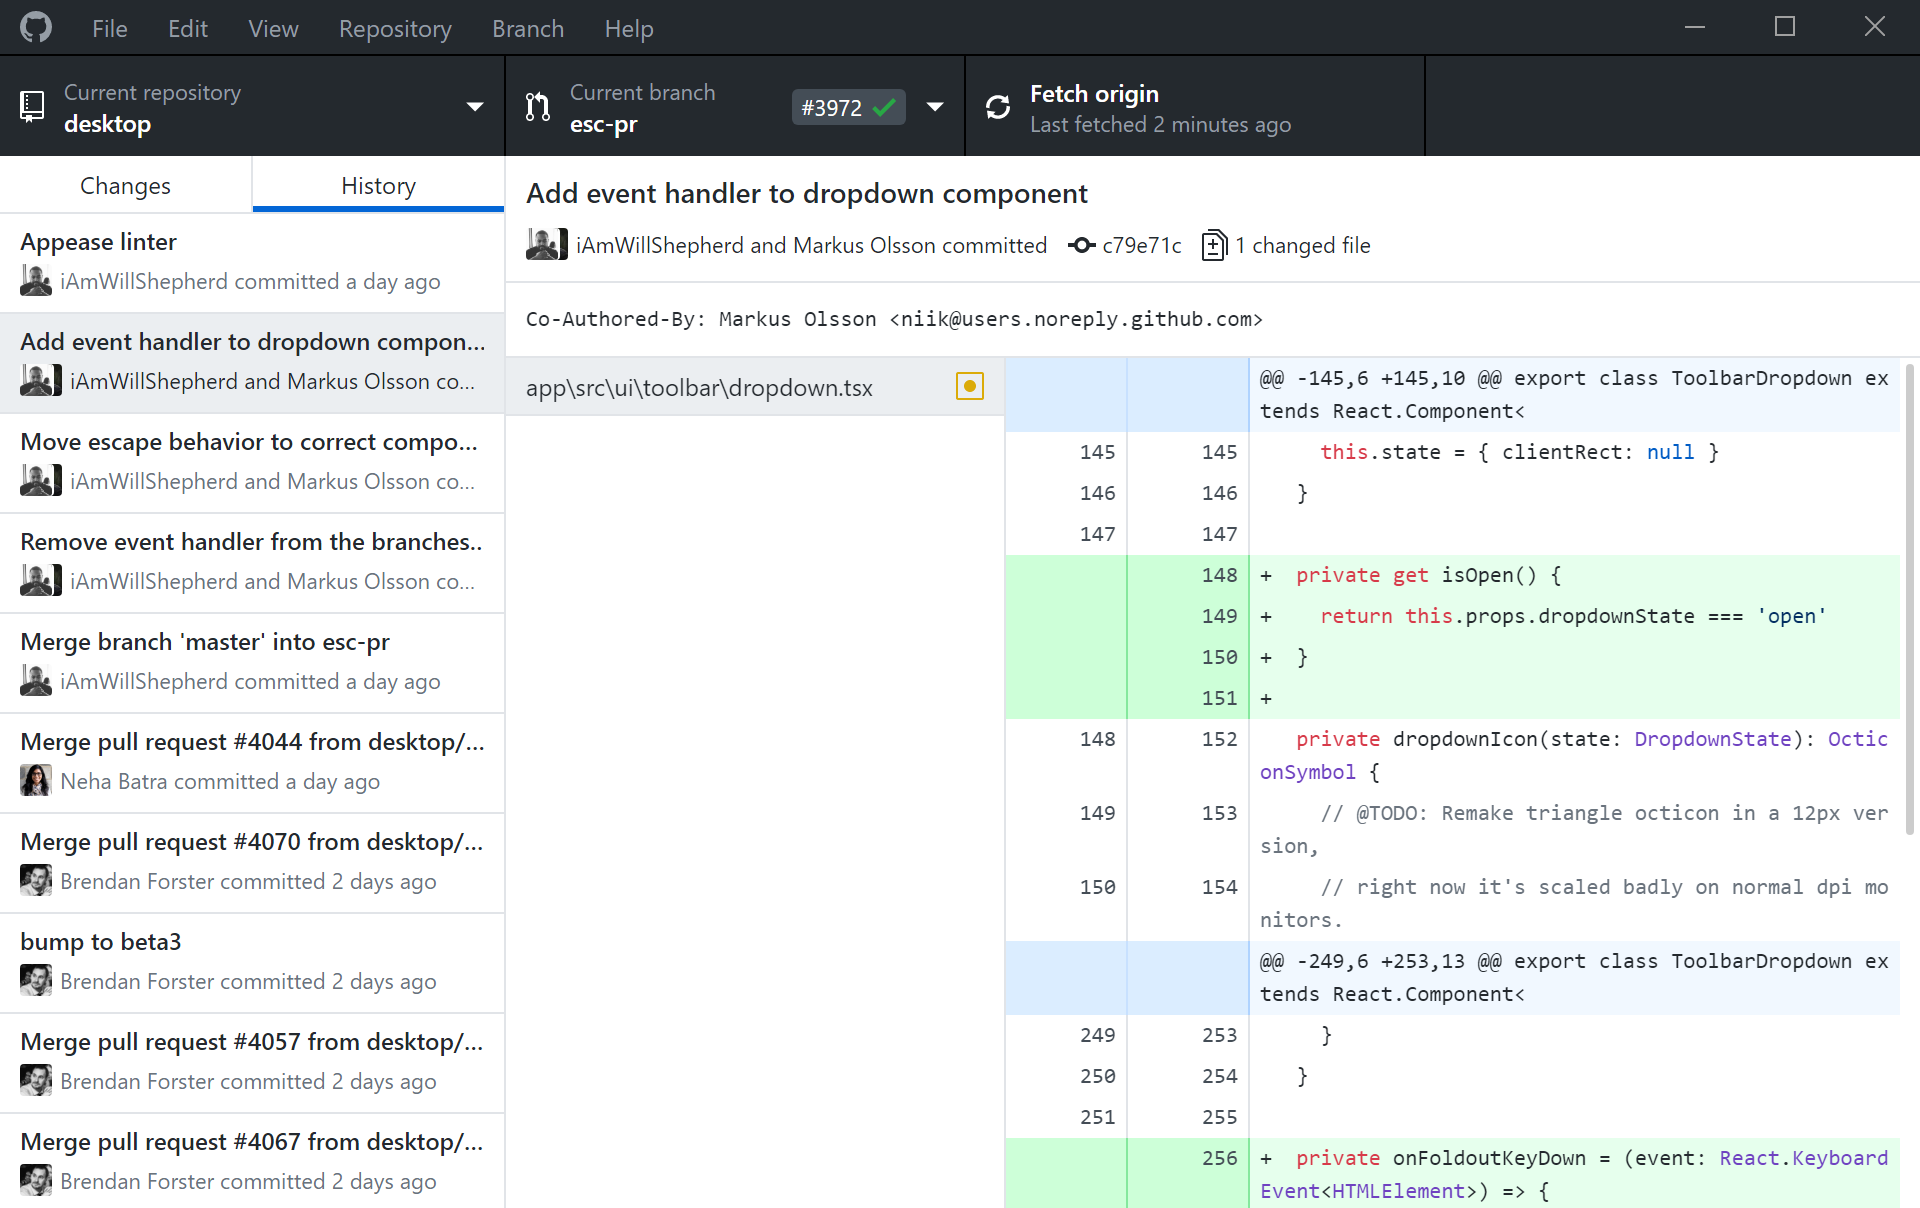
\includegraphics[scale=0.50]{github-desktop}
  \centering
  \caption{Github Desktop в Windows}
  \label{fig:github-desktop}
\end{figure}



\newpage

\section{Разработка}

\subsection{Създаване на проекта}
За да създадем нов Rust проект, първо трябва до отворим конзолата и да изпълним следната команда:
\begin{lstlisting}
cargo new test-generator
\end{lstlisting}

Тя ще генерира папка с името test-generator, в която се намира проекта. В src
папката се намират файловете, в които пишем кода, а в Cargo.toml файла се намира
конфигурацията на проекта.

За да отворим проекта в текстов редактор, може да напишем комантадта `code .` за
да го отворим във VSCode или `nvim .` за да го отворим във Neovim.
 
\begin{figure}[!htb]
  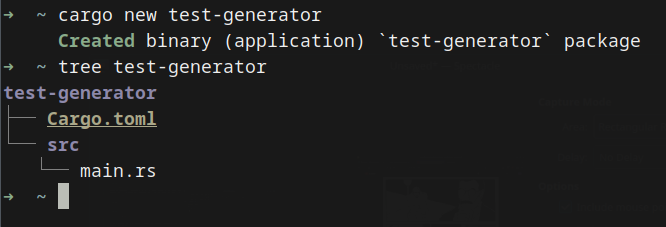
\includegraphics[scale=0.60]{new-rust-project}
  \centering
  \caption{Файловата структура на Rust проекта}
  \label{fig:new-rust-project}
\end{figure}

\subsection{Добавяне на библиотеки}
За да добавим библиотека в Rust трябва да я добавим в Cargo.toml файла под
секцията наречена dependencies. Синтакса за добавяне е много прост, а именно в
ляво името на библиотеката, посредата знака за равно и вдясно версията на
библиотеката.
\begin{figure}[!htb]
  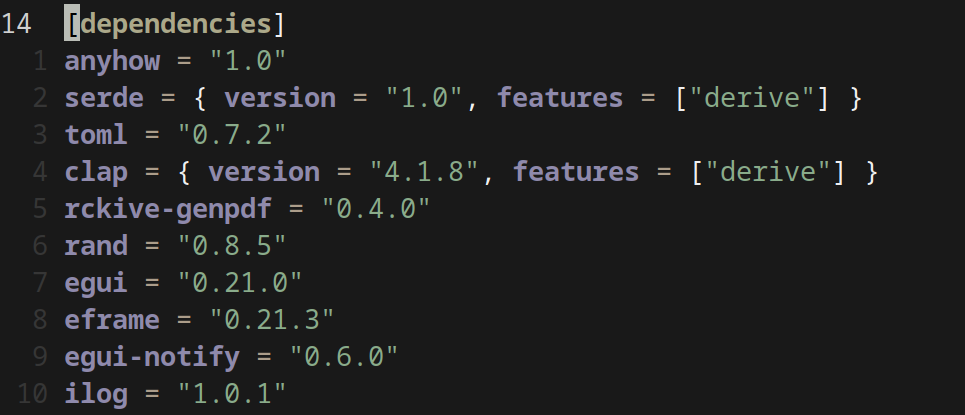
\includegraphics[scale=0.7]{rust-deps.png}
  \centering
  \caption{Ситаксис за добавяне на библиотеки}
  \label{fig:rust-deps}
\end{figure}

\subsubsection{Конзолни аргументи}
Аргументите на конзолата са параметри, предавани на програмата преди изпълнение
и в командния ред. В Rust аргументите могат да бъдат достъпени чрез
функцията \textit{std::env::args()}, която връща итератор над аргументите като списък от
низове.

За да вземем подходящата информация за приложението, може да напишeм наш собствен
анализатор или да изплозваме една от многото различни библиотеки за работа с
конзолни аргументи. Една от най-често използваните библиотеки е \textit{clap} (\textbf{C}onsole \textbf{L}ine
\textbf{A}rgument \textbf{P}arser).

Clap ни предоставя с \textit{clap::Parser} макрото, което при компилирането на програмата
анализира структурата от данни и автоматично търси командните аргументи при
изпълнение на програмата. Също тъка, проверява кои аргументи са маркирани като
задължителни или такива със стойност по подразбиране. [Фигура \ref{fig:clap-example}]
\begin{figure}[!htb]
  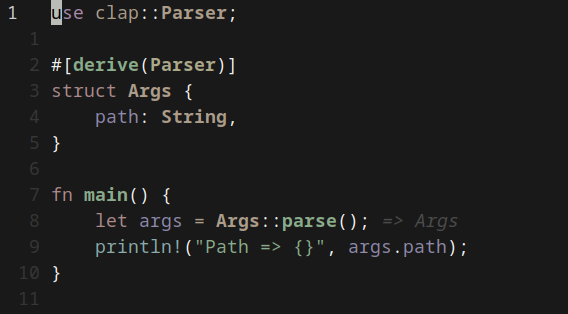
\includegraphics[scale=0.7]{clap-example}
  \centering
  \caption{Четене на командни аргументи с \textit{clap}}
  \label{fig:clap-example}
\end{figure}

При въвеждане на грешни аргументи или при липсата на задължителните такива, \textit{clap}
показва автоматично генерираното помощно съобщение на потребителя.
\begin{figure}[!htb]
  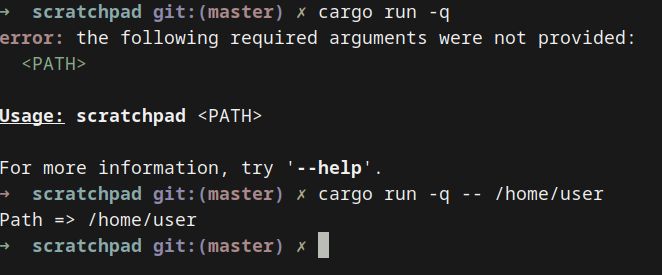
\includegraphics[scale=0.7]{clap-help}
  \centering
  \caption{Генерираното помощно съобщение от \textit{clap}}
  \label{fig:clap-help}
\end{figure}

\subsubsection{Serde}
\textit{Serde} е framework за ефективно сериализиране и десериализиране на структури от данни в Rust.

Екосистемата на \textit{Serde} се състои от структури от данни, които знаят как да
сериализират и десериализират себе си заедно с формата на данните. \textit{Serde} предоставя слой, чрез
който тези две групи взаимодействат помежду си, позволявайки всяка поддържана
структура от данни да бъде сериализирана и десериализирана с помощта на всеки
поддържан формат на данни.

Докато много други езици разчитат на runtime среда (като Dotnet) за
сериализиране на данни, \textit{Serde} вместо това е изградена върху много добрата
интерфес система на Rust.

Структура от данни, която знае как да сериализира и десериализира сама себе си,
е тази, която използва интерфейсите на \textit{Serde} за сериализиране и десериализиране
(или използва атрибута derive на \textit{Serde} за автоматично генериране на интерфеси
по време на компилация). По този начин се избягват забавянето от употребата на
runtime среда.

Всъщност в много ситуации взаимодействието между структурата на данните и
формата на данните може да бъде напълно оптимизирано от Rust компилатора,
оставяйки сериализацията на \textit{Serde} да се изпълни със същата скорост като
ръчно написан сериализатор в езици от по-ниско ниво като \textit{C}.

\subsubsection{Toml}
\textit{Toml} (\textbf{T}om's \textbf{O}bvious \textbf{M}inimal \textbf{L}anguage) е
файлов формат за съхранение на софтуерни конфигурации. Този формат ще бъде
използван за съхраняване на настройките, въпросите и друга информация за
тестовете. За да добавим подръжка за този формат в Rust, трябва да инсталираме
\textit{Toml} библиотека, която използва \textit{Serde} за преобразуването на файл в
обект и обратно.

% TODO: explain how toml is integrated with serde
% TODO: exmaple?

\subsubsection{genpdf}
genpdf е библиотека за генериране на PDF документи на високо ниво, изградена от
две по-малки библиотеки от по-ниско ниво. Тя се грижи за оформлението на
страницата, подравняването на текста и изобразява дървовидната структура на
документа в PDF файла.


% [x] cargo new test-generator
% [x] open in text editor
% [ ] import libraries
%     [x] clap
%     [x] serde
%     [x] toml
%     [x] genpdf
%     [ ] egui
%     [ ] egui-notify
% [ ] create data structures
%     [ ] Project
%         [ ] Question
%             [ ] SelectionQuestion
%             [ ] InputQuestion
% [x] create command line arguments (clap)
%     [x] describe what clap is and how it works
% [ ] create pdf generator
%     [ ] create elements
%         [ ] AlphabeticOrderedList
%         [ ] CharRepeat
%         [ ] SplitElement
%     [ ] setting up the pdf library
%     [ ] generating header
%     [ ] generating questions
%     [ ] generating footer
% [ ] create gui
%     [ ] create questions tab
%     [ ] create configuration tab
%     [ ] create settings tab
% [ ] optimizing builds
% [ ] building for different platforms (MacOS, Windows & Linux)
